\documentclass[%
  a4paper,
  10pt,
  version=last
]{scrartcl}

\usepackage{latex/bilingualagreement/bilingualagreement}

\usepackage{tikz}

% https://eur-lex.europa.eu/legal-content/EN/TXT/HTML/?uri=CELEX:32016R0679
% https://eur-lex.europa.eu/legal-content/DE/TXT/HTML/?uri=CELEX:32016R0679

\begin{document}
  \begin{bilingualagreement}[0.5]
    \addtitle{DSGVO}{GDPR}

    \insertTOCs{Inhaltsverzeichnis}{Table of Contents}

    \medskip

    \begin{listAnnexes}{Anhänge}{Annexes}%[0.25\linewidth][0.05\linewidth][0.25\linewidth]
 	  \addAnnex{Individualvereinbarungsmuster}{Individual Agreement Template}
 	  \addAnnex{Individualvereinbarungsmuster}{Individual Agreement Template}[Label left][Label right] 
    \end{listAnnexes}

    \newpage

    \addsection{GeneralProvisions}{Allgemeine Bestimmungen}{General Provisions}

    \addclause{SubjectMatter}{Gegenstand und Ziele}{Subject Matter}{
      \begin{enumerate}[(1)]
        \item Diese Verordnung enthält Vorschriften zum Schutz natürlicher
        Personen bei der Verarbeitung personenbezogener Daten und zum freien
        Verkehr solcher Daten.
        \item Diese Verordnung schützt die Grundrechte und Grundfreiheiten
        natürlicher Personen und insbesondere deren Recht auf Schutz
        personenbezogener Daten.
        \item Der freie Verkehr personenbezogener Daten in der Union darf aus
        Gründen des Schutzes natürlicher Personen bei der Verarbeitung
        personenbezogener Daten weder eingeschränkt noch verboten werden.
      \end{enumerate}
    }{
      \begin{enumerate}[(1)]
        \item This Regulation lays down rules relating to the protection of
        natural persons with regard to the processing of personal data and rules
        relating to the free movement of personal data.
        \item This Regulation protects fundamental rights and freedoms of natural
        persons and in particular their right to the protection of personal data.
        \item The free movement of personal data within the Union shall be
        neither restricted nor prohibited for reasons connected with the
        protection of natural persons with regard to the processing of personal
        data.
      \end{enumerate}
    }

    \addfigure{%
      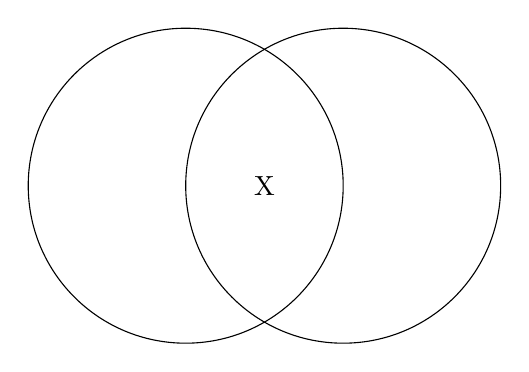
\begin{tikzpicture}
        \draw (0,0) circle (2cm);
        \draw (2,0) circle (2cm);
        \node at (1,0) {X};
      \end{tikzpicture}
    }{Mengendiagramm}{Venn diagram}

    \addclause{MaterialScope}{Sachlicher Anwendungsbereich}{Material scope}{
      \begin{enumerate}[(1)]
        \item Diese Verordnung gilt für die ganz oder teilweise automatisierte
          Verarbeitung personenbezogener Daten sowie für die nichtautomatisierte
          Verarbeitung personenbezogener Daten, die in einem Dateisystem
          gespeichert sind oder gespeichert werden sollen.
        \item Diese Verordnung findet keine Anwendung auf die Verarbeitung
          personenbezogener Daten
          \begin{enumerate}[a)]
            \item im Rahmen einer Tätigkeit, die nicht in den Anwendungsbereich
              des Unionsrechts fällt,
            \item durch die Mitgliedstaaten im Rahmen von Tätigkeiten, die in den
              Anwendungsbereich von Titel V Kapitel 2 EUV fallen,
            \item durch natürliche Personen zur Ausübung ausschließlich
              persönlicher oder familiärer Tätigkeiten,
            \item durch die zuständigen Behörden zum Zwecke der Verhütung,
              Ermittlung, Aufdeckung oder Verfolgung von Straftaten oder der
              Strafvollstreckung, einschließlich des Schutzes vor und der Abwehr
              von Gefahren für die öffentliche Sicherheit.
          \end{enumerate}
        \item Für die Verarbeitung personenbezogener Daten durch die Organe,
          Einrichtungen, Ämter und Agenturen der Union gilt die Verordnung (EG)
          Nr. 45/2001. Die Verordnung (EG) Nr. 45/2001 und sonstige Rechtsakte
          der Union, die diese Verarbeitung personenbezogener Daten regeln,
          werden im Einklang mit Artikel 98 an die Grundsätze und Vorschriften
          der vorliegenden Verordnung angepasst.
        \item Die vorliegende Verordnung lässt die Anwendung der Richtlinie
          2000/31/EG und speziell die Vorschriften der Artikel 12 bis 15 dieser
          Richtlinie zur Verantwortlichkeit der Vermittler unberührt.
      \end{enumerate}
    }{
      \begin{enumerate}[(1)]
        \item This Regulation applies to the processing of personal data wholly
          or partly by automated means and to the processing other than by
          automated means of personal data which form part of a filing system or
          are intended to form part of a filing system.
        \item This Regulation does not apply to the processing of personal data:
          \begin{enumerate}[a)]
            \item in the course of an activity which falls outside the scope of Union law;
            \item by the Member States when carrying out activities which fall
              within the scope of Chapter 2 of Title V of the TEU;
            \item by a natural person in the course of a purely personal or
              household activity;
            \item by competent authorities for the purposes of the prevention,
              investigation, detection or prosecution of criminal offences or the
              execution of criminal penalties, including the safeguarding against
              and the prevention of threats to public security.
          \end{enumerate}
        \item For the processing of personal data by the Union institutions,
          bodies, offices and agencies, Regulation (EC) No 45/2001 applies.
          Regulation (EC) No 45/2001 and other Union legal acts applicable to
          such processing of personal data shall be adapted to the principles and
          rules of this Regulation in accordance with Article 98.
        \item This Regulation shall be without prejudice to the application of
          Directive 2000/31/EC, in particular of the liability rules of
          intermediary service providers in Articles 12 to 15 of that Directive.
      \end{enumerate}
    }
  \end{bilingualagreement}
\end{document}
